\documentclass[a4paper]{article}

\usepackage[english]{babel}
\usepackage{graphicx}
\usepackage{wrapfig}
%\usepackage[caption=false,font=normalsize,
%labelfont=sf,textfont=sf]{subfig}
\usepackage[font=normalsize,labelfont=sf,textfont=sf]{subcaption} % Use only subcaption, not subfig

\usepackage{geometry}
\geometry{left=0cm,right=0cm,top=0.2cm,bottom=0.2cm}

\begin{document}
	
	\begin{figure*}
		\centering % 将整个 figure* 居中
		\begin{subfigure}{0.95\linewidth}
			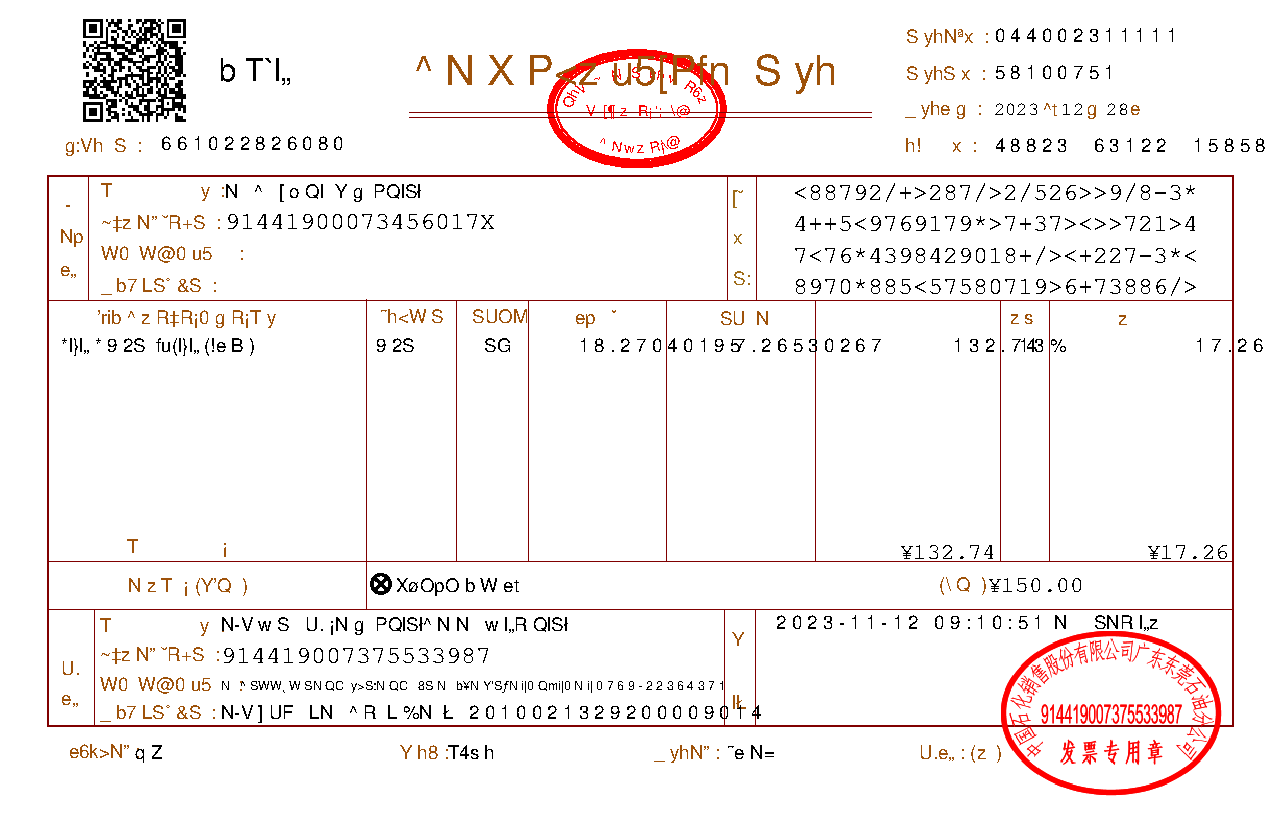
\includegraphics[width=\linewidth]{software/1}
			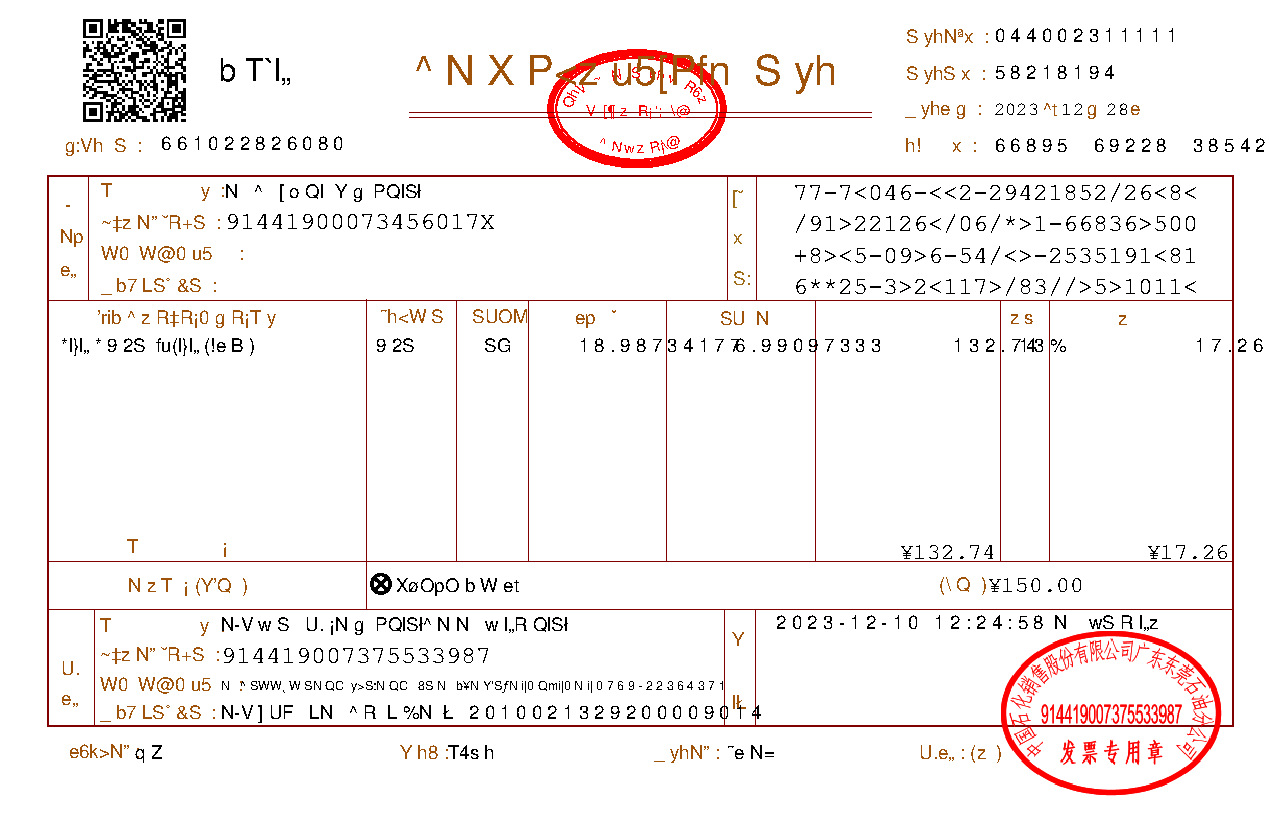
\includegraphics[width=\linewidth]{software/2}
		\end{subfigure}
	\end{figure*} 
	
	
	\begin{figure*}
		\centering % 将整个 figure* 居中
		\begin{subfigure}{0.95\linewidth}
			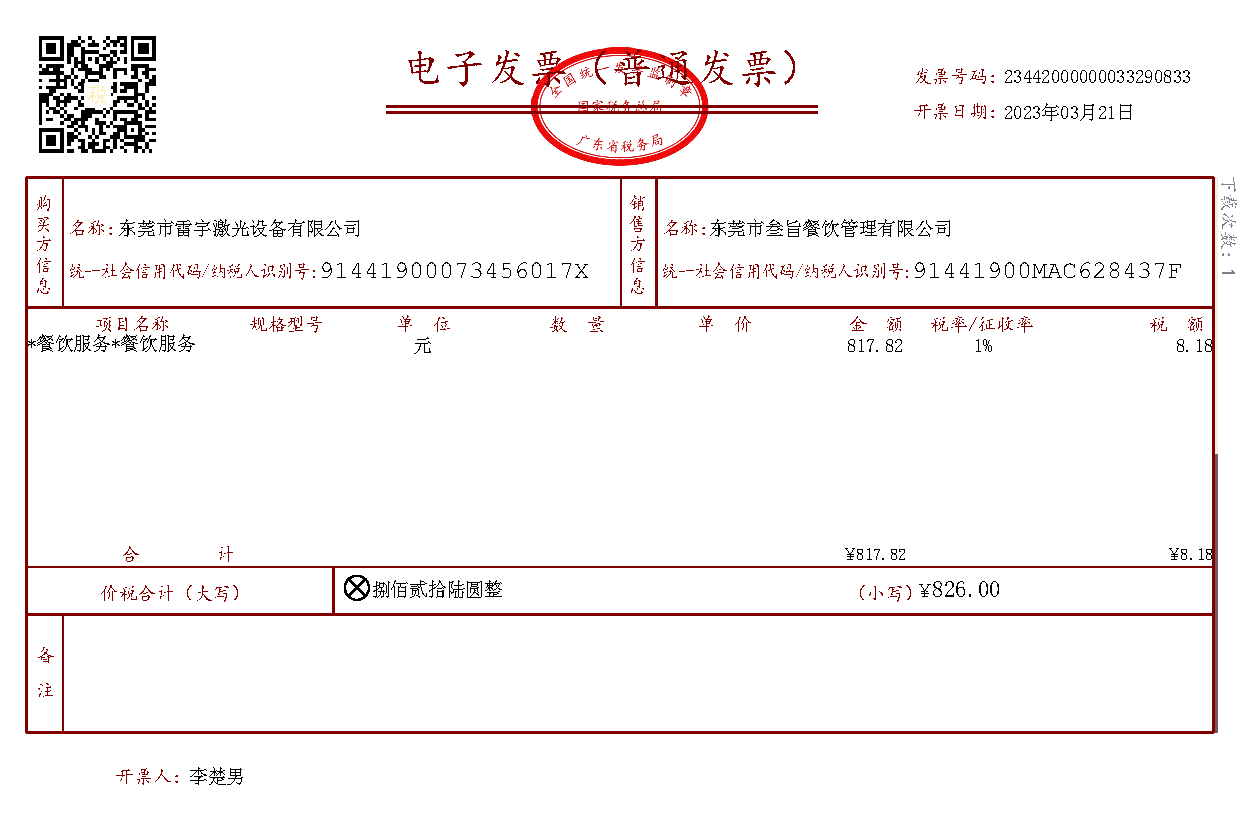
\includegraphics[width=\linewidth]{software/3}
			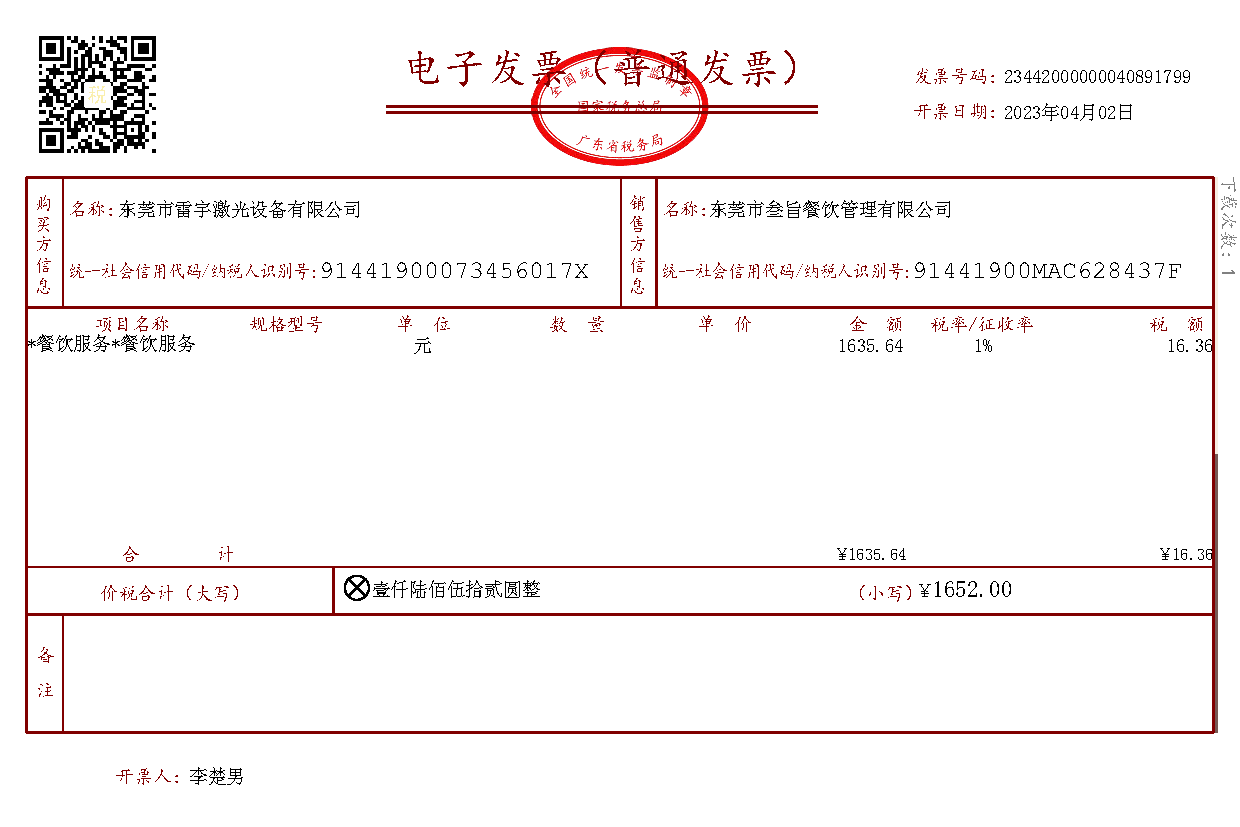
\includegraphics[width=\linewidth]{software/4}
		\end{subfigure}
	\end{figure*} 
	
	\begin{figure*}
		\centering % 将整个 figure* 居中
		\begin{subfigure}{0.95\linewidth}
			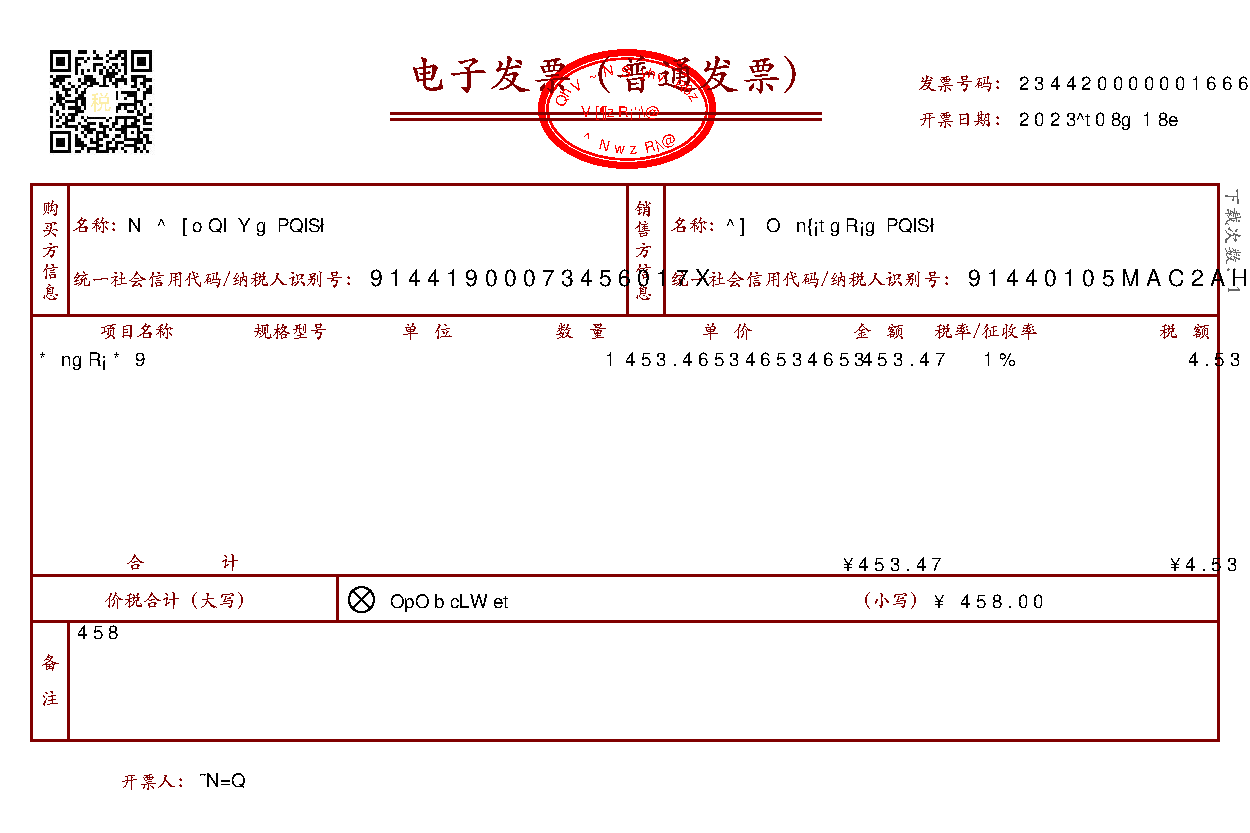
\includegraphics[width=\linewidth]{software/5}
			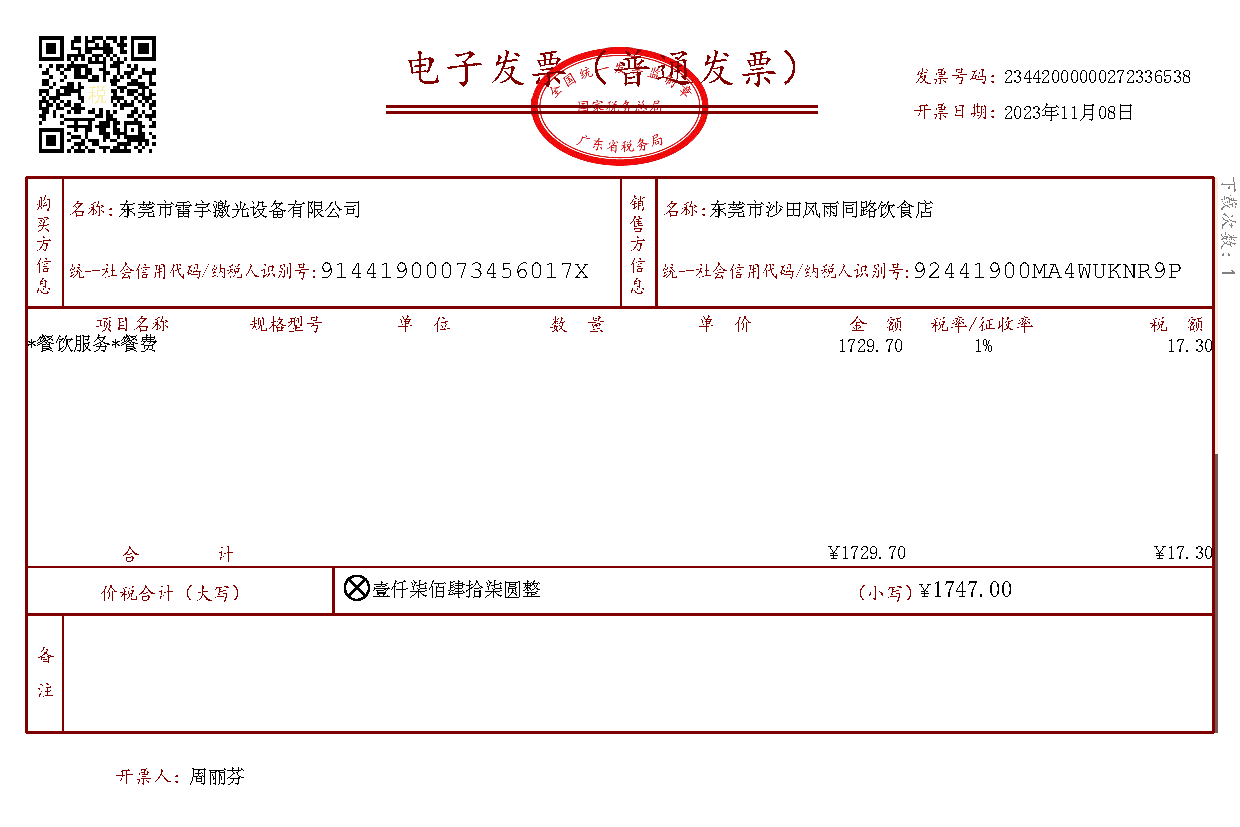
\includegraphics[width=\linewidth]{software/6}
		\end{subfigure}
	\end{figure*} 
	
	\begin{figure*}
		\centering % 将整个 figure* 居中
		\begin{subfigure}{0.95\linewidth}
			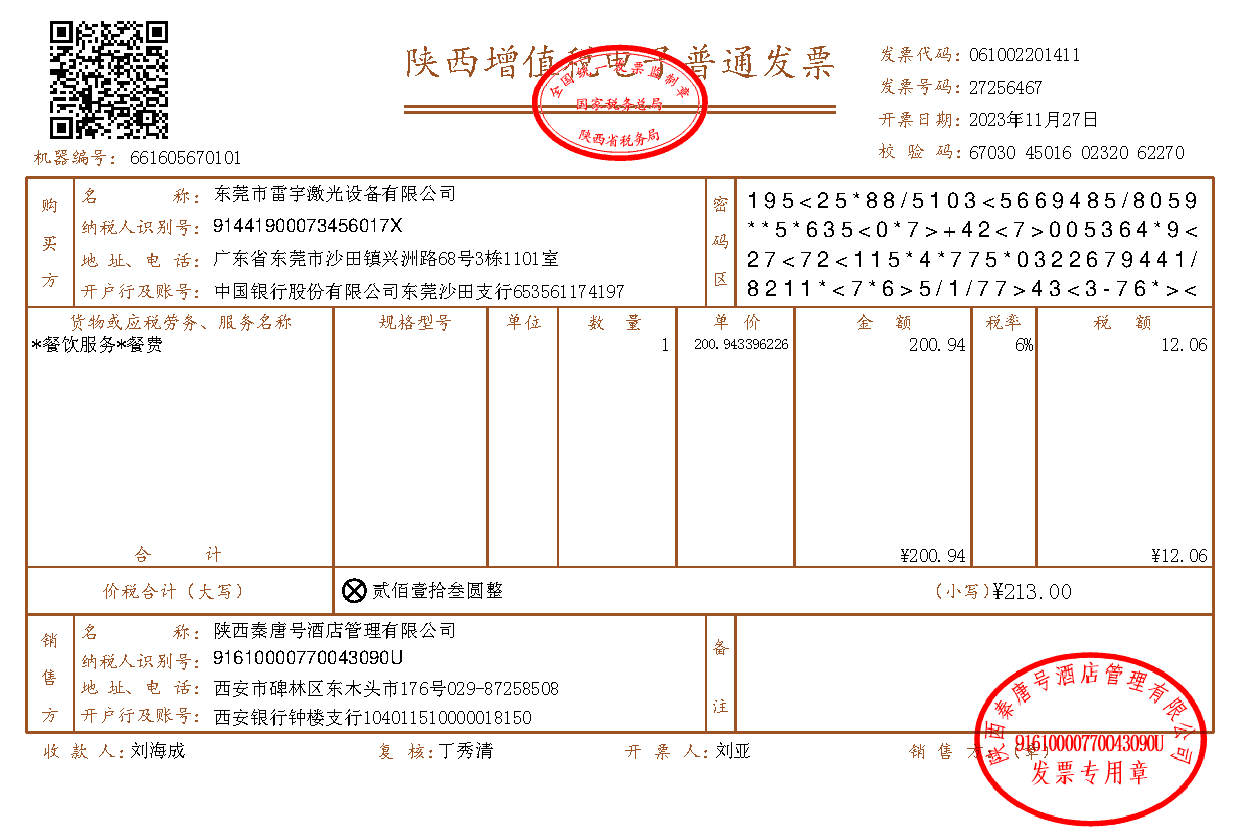
\includegraphics[width=\linewidth]{software/7}
			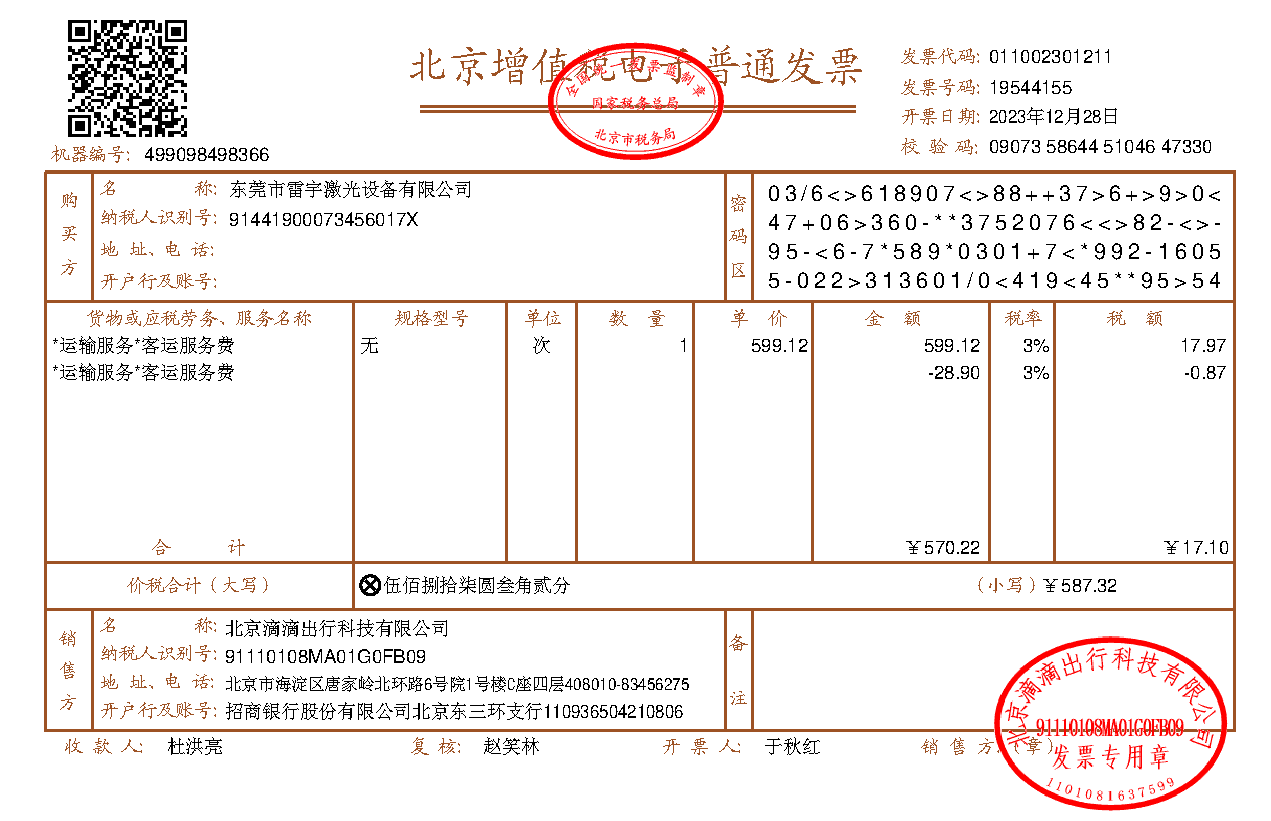
\includegraphics[width=\linewidth]{software/8}
		\end{subfigure}
	\end{figure*} 
	
	\begin{figure*}
		\centering % 将整个 figure* 居中
		\begin{subfigure}{0.95\linewidth}
			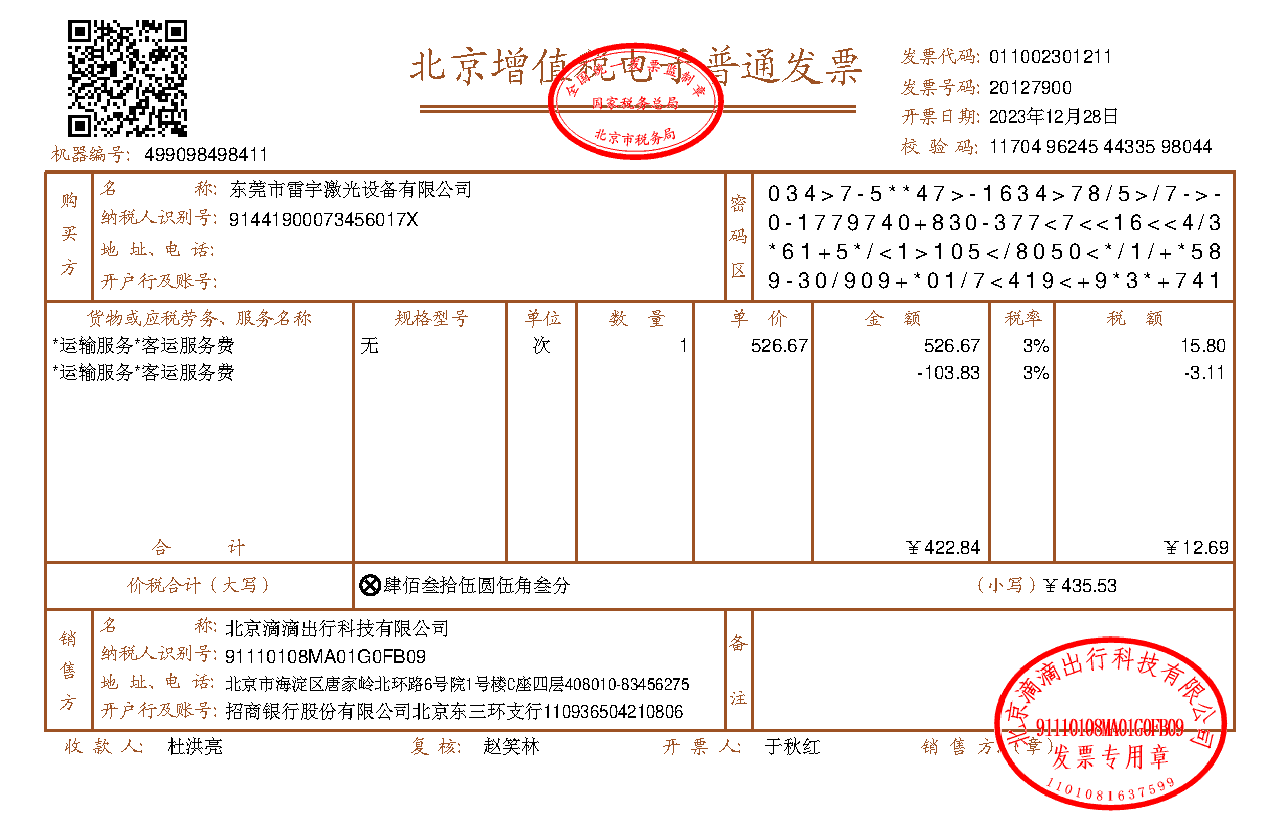
\includegraphics[width=\linewidth]{software/9}
		\end{subfigure}
	\end{figure*} 
\end{document}